\begin{table}[H]
	\centering
	\begin{tabular}{rlrlll}
		\toprule
			& \multicolumn{2}{c}{
        \textbf{Parameter values}
        }
        &&&
        \multicolumn{1}{c}{\textbf{Initial Conditions}}
        \\
      \cmidrule{1-4}
      \cmidrule{6-6}
        $\beta_1$ 
            & \num{13.0}            
        &
        $\beta_2$ 
        & \num{13.0}
        &&
          $S(0) = (76/120)N$
          \\
        $\beta_3$ 
          & \num{0.0131}, 
            \num{0.0217},
        &&
        &&
          $L_1(0) = (36/120) N$
          \\
          & \num{0.029}, 
            \num{0.0436}
          &&&&
            $L_2(0) =(2/120) N$
        \\
          &&
          &&&
          $I_1(0) = (4/120)N$
        \\
        $\mu$ 
          & \num{0.0143}
          &&&&
          $I_2(0) = (1/120)N$
        \\
     	$d_1$ 
          & \num{0.0}
      &
      $d_2$ 
          & \num{0.0}
          &&
            $T(0)= (1/120)N$
     \\
     	$k_1$ 
      & \num{0.5}
      &
       $k_2$  
      & \num{1.0}
      \\
      $r_1$ 
      & \num{2.0}
      &
    $r_2$ 
      & \num{1.0}
      \\
    $p$
      & \num{0.4}
      &
      $q$
      & \num{0.1}
    \\
      $N$
      & 
        \num{6000}, 
        \num{12000}, 
      &
      $\Lambda$ 
      & $\mu N$
      \\
      &
      \num{30000}
      &&&&
      \multicolumn{1}{c}{\textbf{Control Bounds}}
      \\
      \cmidrule{6-6}
      &&&&&
        Lower \num{0.05}
      \\
      &&&&&
        Upper \num{0.95}s
      \\
      $t_f$ 
      &
        \SI{5.0}{years}
      \\
      $B_1$ 
        & \num{50.0}
      &
      $B_2$
      & \num{500.0}
      & 
      \\
      \bottomrule
    \end{tabular}
	\caption{Simulation values for the control 
	problem \eqref{eqn:MDR-TB_model}.}
	\label{tbl:parameters_MDR-TB_model}
\end{table}
%
	\Cref{fig:figure1twostraintbm} shows the effect of case finding and 
case holding controls. The combination of this strategies diminish the multi 
drug resistant population. \Cref{tbl:parameters_MDR-TB_model} compiles the 
parameters and its values used to produce this figure and fix 
$N = \num{30000}$, $\beta_3 = \num{0.29}$. To minimize the resistant TB 
population, L2 + I2, the simulation suggest that the case holding strategy 
$u_2$ would be at the upper bound during almost \SI{4.3}{years} and then 
decreasing to the lower bound. Meanwhile, decreasing value for case finding
must apply over the most of the simulated time, \SI{5}{years}. The total number 
of 
infected resistant TB $L2 + I2$  at the final time $t_f = \SI{5}{years}$ results
\num{1123}. This same number but without control sums 4176. So this policies 
prevents \SI{3053}{cases} of resistant TB.

  According with \Cref{tbl:parameters_MDR-TB_model} and taking different values
for the parameter $\beta_3$, in \Cref{fig:figure2twostraintbm} we illustrate 
the effect of parameter $\beta_3$ over controls.The 
simulation suggest that both controls experiment small variations just at the 
beginning and reach almost the same level after \SI{5}{year}. As wee see the 
simulation suggest that just delay the same profile for few months.
%
\begin{figure}[H]
  \centering
  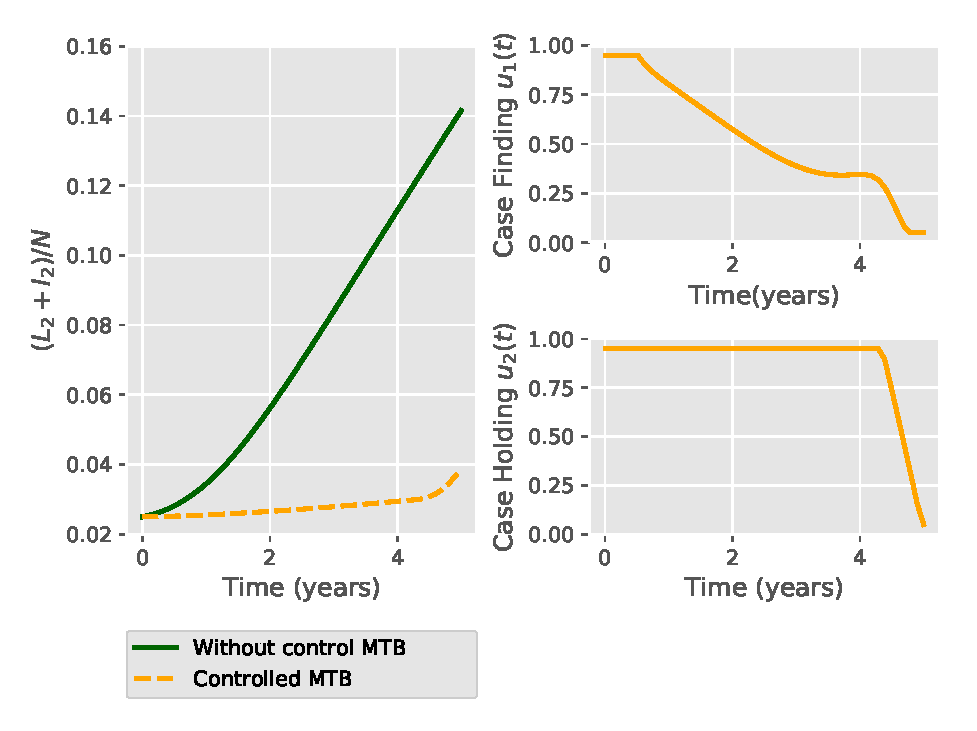
\includegraphics{Figures/figure_1_two_strain_tbm}
  \caption{Normalized infected population according to parameters of 
  \Cref{tbl:parameters_MDR-TB_model}. Here the green line represents the 
  infected population without control. As we see, combining case finding 
  $u_1(t)$ and  case holding $u_2(t)$, dramatically diminish the density of 
  infected with resistant TB.}
  \label{fig:figure1twostraintbm}
\end{figure}

%
\begin{figure}[H]
  \centering
  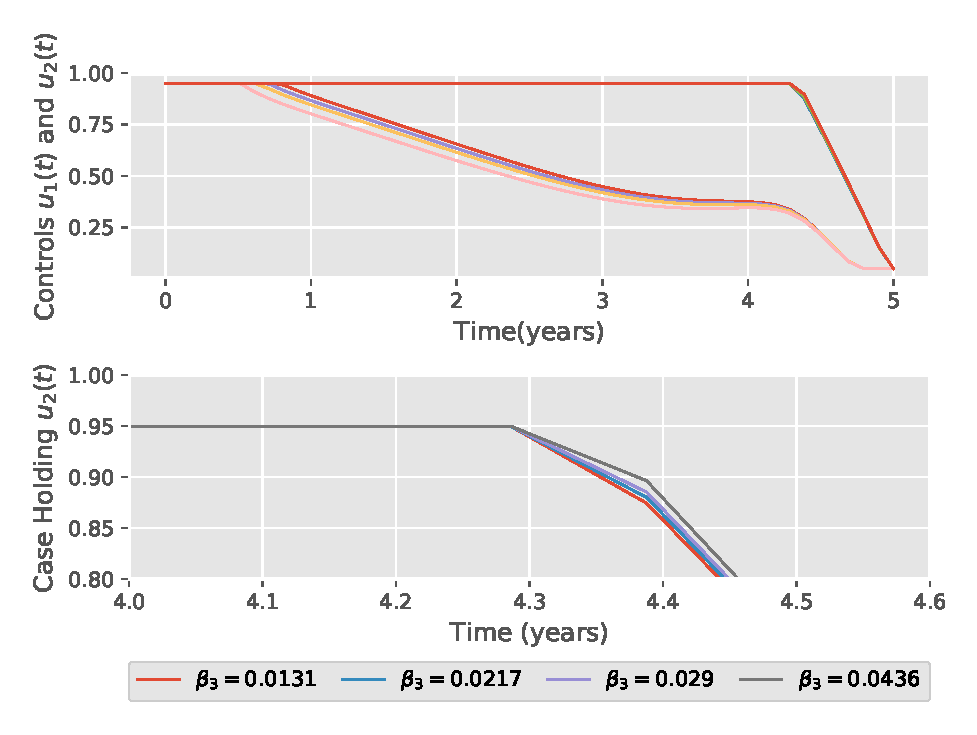
\includegraphics{Figures/figure_2_two_strain_tbm}
  \caption{
    Top case finding and case holding controls 
    under parameters encased in \Cref{tbl:parameters_MDR-TB_model} and
    different values of parameter $\beta_3$. At bottom we capture a smaller
    region to illustrate the variations regarding to case holding. Simulation 
    suggest 
    that case holding remains almost with the same profile, while case finding 
    delays same period for only for a few months.
  }\label{fig:figure2twostraintbm}
\end{figure}

\Cref{fig:figure3twostraintbm} illustrates case finding and case holding 
strategies under population of different sizes. The simulation suggest that
under relative small population, is more important holds case finding at the 
top. While for relatively bigger population the case holding is the more 
important strategy.
\begin{figure}[H]
  \centering
  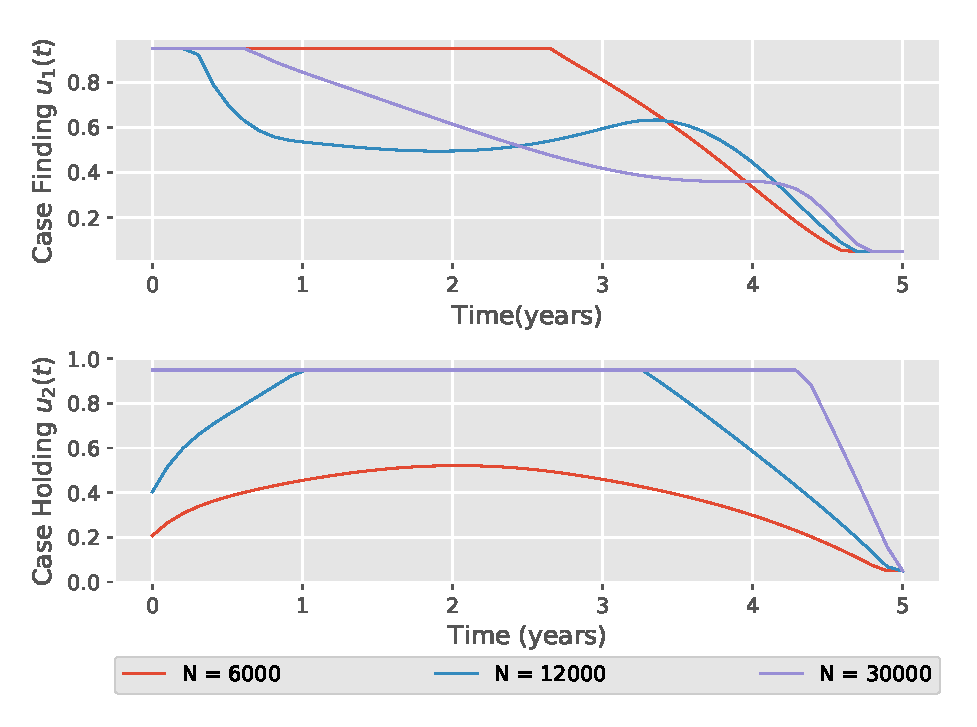
\includegraphics{Figures/figure_3_two_strain_tbm}
  \caption{
    The effect of different size of populations. For 
    relatively small population, the case finding strategy is more important 
    than case finding, meanwhile for  bigger populations, the case holding 
    plays a more important role. The rest of parameters as in 
    \Cref{tbl:parameters_MDR-TB_model}.
  }
  \label{fig:figure3twostraintbm}
\end{figure}
